\documentclass{article}\usepackage[]{graphicx}\usepackage[]{color}
%% maxwidth is the original width if it is less than linewidth
%% otherwise use linewidth (to make sure the graphics do not exceed the margin)
\makeatletter
\def\maxwidth{ %
  \ifdim\Gin@nat@width>\linewidth
    \linewidth
  \else
    \Gin@nat@width
  \fi
}
\makeatother

\definecolor{fgcolor}{rgb}{0.345, 0.345, 0.345}
\newcommand{\hlnum}[1]{\textcolor[rgb]{0.686,0.059,0.569}{#1}}%
\newcommand{\hlstr}[1]{\textcolor[rgb]{0.192,0.494,0.8}{#1}}%
\newcommand{\hlcom}[1]{\textcolor[rgb]{0.678,0.584,0.686}{\textit{#1}}}%
\newcommand{\hlopt}[1]{\textcolor[rgb]{0,0,0}{#1}}%
\newcommand{\hlstd}[1]{\textcolor[rgb]{0.345,0.345,0.345}{#1}}%
\newcommand{\hlkwa}[1]{\textcolor[rgb]{0.161,0.373,0.58}{\textbf{#1}}}%
\newcommand{\hlkwb}[1]{\textcolor[rgb]{0.69,0.353,0.396}{#1}}%
\newcommand{\hlkwc}[1]{\textcolor[rgb]{0.333,0.667,0.333}{#1}}%
\newcommand{\hlkwd}[1]{\textcolor[rgb]{0.737,0.353,0.396}{\textbf{#1}}}%

\usepackage{framed}
\makeatletter
\newenvironment{kframe}{%
 \def\at@end@of@kframe{}%
 \ifinner\ifhmode%
  \def\at@end@of@kframe{\end{minipage}}%
  \begin{minipage}{\columnwidth}%
 \fi\fi%
 \def\FrameCommand##1{\hskip\@totalleftmargin \hskip-\fboxsep
 \colorbox{shadecolor}{##1}\hskip-\fboxsep
     % There is no \\@totalrightmargin, so:
     \hskip-\linewidth \hskip-\@totalleftmargin \hskip\columnwidth}%
 \MakeFramed {\advance\hsize-\width
   \@totalleftmargin\z@ \linewidth\hsize
   \@setminipage}}%
 {\par\unskip\endMakeFramed%
 \at@end@of@kframe}
\makeatother

\definecolor{shadecolor}{rgb}{.97, .97, .97}
\definecolor{messagecolor}{rgb}{0, 0, 0}
\definecolor{warningcolor}{rgb}{1, 0, 1}
\definecolor{errorcolor}{rgb}{1, 0, 0}
\newenvironment{knitrout}{}{} % an empty environment to be redefined in TeX

\usepackage{alltt}
\usepackage{Sweave}
\usepackage{graphicx}
\usepackage{tabularx}
\usepackage[small]{caption}
\usepackage{gensymb}
\usepackage{float}
\usepackage{subfig}
\usepackage{url}
\setkeys{Gin}{width=0.8\textwidth}
\setlength{\captionmargin}{30pt}
\setlength{\abovecaptionskip}{0pt}
\setlength{\belowcaptionskip}{10pt}
\topmargin -1.5cm        
\oddsidemargin -0.04cm   
\evensidemargin -0.04cm
\textwidth 16.59cm
\textheight 21.94cm 
\pagestyle{empty}
\parskip 7.2pt
\renewcommand{\baselinestretch}{1.5}
\parindent 0pt
\IfFileExists{upquote.sty}{\usepackage{upquote}}{}
\begin{document}

\renewcommand{\thetable}{\arabic{table}}
\renewcommand{\thefigure}{\arabic{figure}}
\renewcommand{\labelitemi}{$-$}
%%%%%%%%%%%%%%%%%%%%%%%%%%%%%%%%%%%%%%%%%%%%%%%%%%%%%%%
{\huge\textbf{\textit{Carya glabra}}}

\section*{Overview}
The pignut hickory is part of the Walnut family, or the Juglandaceae family. It is a medium to large sized tree, roughly 60-80 feet tall (18-24m) and has a trunk diameter of 1-2 feet (0.3-0.6m). The canopy width is generally 25-40 feet (7-12m). The pignut hickory typically grows in dry and moist uplands in hardwood forests in communities of oaks and other hickory trees and blooms around April or May. 
\section*{Habitat and Growth}
The pignut hickory grows best in rich, medium moisture soil that is well-drained and in an area that receives full to partial sun. The tree requires a lot of space to grow and is difficult to transplant due to its long taproot. It is commonly found on ridges or hillslopes and is most prevalent along the Appalachian forests and the lower Ohio River Basin. The pignut hickory does not have any serious insect or disease problems, however the hickory bark beetle, weevils,  and borers can occassionally cause damage in certain regions of the range. The pignut hickory is not known as an ornamental tree but it is commonly planted within large properties or parks for shade. The range can be seen in Figure 1. Given the wide range and distribution of the species, it can grow in temperatures ranging from -30\degree{C} to 46\degree{C} (-22 to 115\degree{F}). Although the growing season will vary by latitude and elevation. Pignut hickories are a common species but not generally abundant. They are often found in upland climax forests alongside other hickory species and oak species. 
\subsection*{Reproduction and Propogation}
Pignut hickories are monoecious. Flowers open starting from the middle of March in the southeast to early June around the northeastern region of the range. The fruit is pear shaped and enclosed in a thin husk. It ripens around September and October and seeds are dispered from September through December. 
\begin{figure}[ht]%
    \centering
    \subfloat[Pignut Hickory Fruit]{{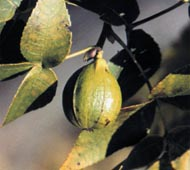
\includegraphics[width=7cm]{fruit.jpg} }}%
    \qquad
    \subfloat[Ripe Pignut Hickory Fruit]{{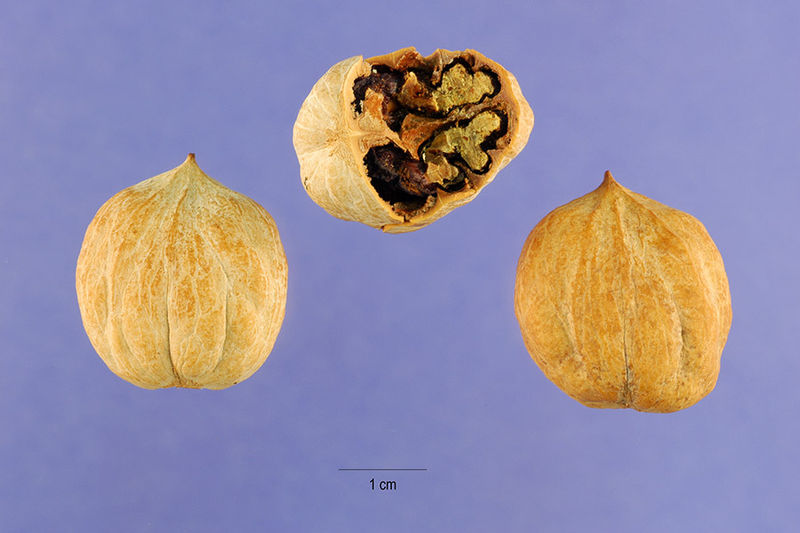
\includegraphics[width=7cm]{ripe_pignut.jpg} }}%
    \caption{Pignut Hickor Fruit Phenophases}%
    \label{fig:example}%
\end{figure}

\begin{figure}[ht]
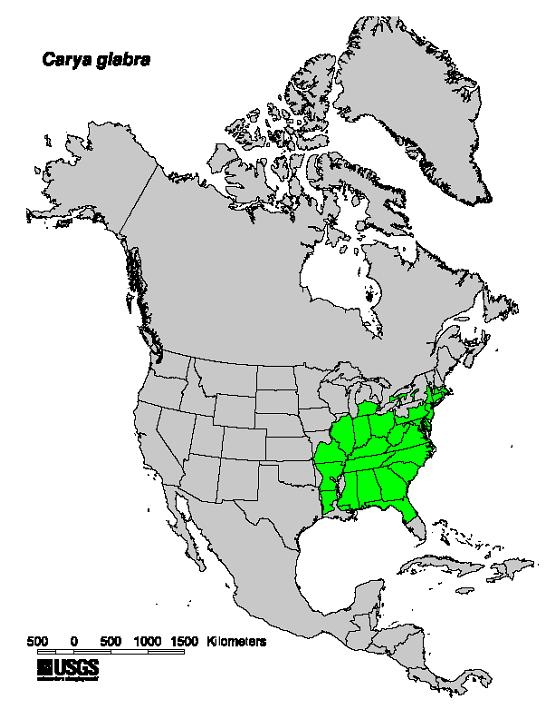
\includegraphics[width=0.5\textwidth]{Carya_glabra_range_map.jpg}
\centering
\caption{Distribution map of \textit{Carya glabra} throughout North America}
\end{figure}

\section{References}
\url{http://dendro.cnre.vt.edu/dendrology/syllabus/factsheet.cfm?ID=19} \\
\url{http://plants.usda.gov/core/profile?symbol=cagl8} \\
\url{http://www.missouribotanicalgarden.org/PlantFinder/PlantFinderDetails.aspx?kempercode=d376} \\
\url{https://www.na.fs.fed.us/pubs/silvics_manual/volume_2/carya/glabra.htm} \\



\end{document}
